
%********************************************************************************************
%											Details
%********************************************************************************************
\title{B.E. Report}
\author{Akshay Chavan}
\date{14.08.2021}
%********************************************************************************************
%											Packages
%********************************************************************************************

\documentclass{report} %defining document class

\usepackage[a4 paper, margin=1in]{geometry} %for page setup
\usepackage{tikz} %for page borders
\usetikzlibrary{calc} %for page borders
\newcommand\HRule{\rule{\textwidth}{1pt}} %for page borders
\usepackage{fancyhdr} %for header and footer
\pagestyle{fancy} 	  %for header and footer
\usepackage{setspace} %for typeset the document with double linespacing
\usepackage{multicol} %for multi-columns
\usepackage{graphicx} %for images
\usepackage{ragged2e} %for text alignment
\usepackage{multirow} %for merging multiple rows
\usepackage[titletoc]{appendix} %for appendix renaming
\usepackage{float} %for "H" parameter in the table
\usepackage{xcolor, colortbl} %for coloring a specific cell in a table
\usepackage{url} %for displaying a url


\setcounter{secnumdepth}{3} %for subsubsection of ToC
\setcounter{tocdepth}{3}    %for subsubsection of ToC

\usepackage{lipsum}         %for dummy text
\usepackage[english]{babel} %for dummy text

\fancypagestyle{front}{ %header and footer style for TOC, LOF, LOT
	\fancyhf{}
	\renewcommand{\headrulewidth}{0pt}
	\renewcommand{\footrulewidth}{0pt}
	\cfoot{\thepage}
	}
\makeatletter
\newcommand\frontpagestyle{\cleardoublepage\pagestyle{front}\let\ps@plain\ps@front}
\makeatother

\usepackage{color}   %May be necessary if you want to color links
\usepackage{hyperref} %for hypertext
\hypersetup{
	%linkcolor=blue,  %set any color for hyperlink in TOC, LOF, LOT.
	%colorlinks=true, %set "true" for colored hyperlink in TOC, LOF, LOT
	linktoc=all       %set "all" for both sections and subsections hyperlink
	}

%********************************************************************************************
%										Title Page
%********************************************************************************************

\begin{document}
		
	\begin{titlepage} 
		
		\begin{tikzpicture}[remember picture, overlay]
			\draw[line width = 1pt] ($(current page.north west) + (0.5in,-0.5in)$) 
			rectangle ($(current page.south east) + (-0.5in,0.5in)$);
		\end{tikzpicture}
		
		\begin{center}
			\large
			\textbf {A PROJECT REPORT ON} \\
			\vspace{1cm}
			
			\Large
			\textbf {YOUR AWESOME PROJECT REPORT TITLE GOES HERE} \\
			\vspace{1cm}
			
			\large
			SUBMITTED TO THE SAVITRIBAI PHULE PUNE UNIVERSITY, PUNE \\
			IN THE PARTIAL FULFILLMENT OF THE REQUIREMENTS \\
			FOR THE AWARD OF THE DEGREE \\
			\vspace{1cm}
			
			\textbf {BACHELOR OF ENGINEERING} \\
			\textbf {(Computer Engineering)} \\
			\vspace{0.5cm}
			
			\textbf {BY} \\
			\vspace{0.5cm}
			
			\begin{tabular}{ll}
				Student 1 & B120484221 \\
				Student 2 & B120484221 \\
				Student 3 & B120484221 \\
				Student 4 & B120484221 \\
			\end{tabular}
			\vspace{0.5cm}
			
			\textbf {Under The Guidance of} \\
			\vspace{0.5cm}
			
			Prof. Guide's name
			\vspace{1cm}
			
			
\includegraphics[scale=0.1]{images/college logo.jpg}
			\vspace{1cm}
			
			\textbf {DEPARTMENT OF COMPUTER ENGINEERING} \\
			\vspace{0.5cm}
			
			\textbf {COLLEGE OF ENGINEERING PUNE (COEP)} \\
			Shivajinagar, Pune - 411005. \\
			\vspace{2cm}
			
			\textbf {SAVITRIBAI PHULE PUNE UNIVERSITY, PUNE} \\
			\vspace{0.5cm}
			
			\textbf {2021 - 2022}
		\end{center}
	
	\end{titlepage}	

%********************************************************************************************
%											Certificate
%********************************************************************************************
	
	\begin{titlepage} 
		
		\begin{tikzpicture}[remember picture, overlay]
			\draw[line width = 1pt] ($(current page.north west) + (0.5in,-0.5in)$) 
			rectangle ($(current page.south east) + (-0.5in,0.5in)$);
		\end{tikzpicture}
		
		\begin{center}
			
\includegraphics[scale=0.1]{images/college logo.jpg}
			\vspace{1cm}
			
			\Large
			\textbf {CERTIFICATE} \\
			\vspace{0.5cm}
			
			\large
			This is to certify that the Project Entitled \\
			\Large
			\textbf {YOUR AWESOME PROJECT REPORT TITLE GOES HERE} \\
			\vspace{0.5cm}
			
			\large
			Submitted by \\
			\vspace{0.5cm}
			
			\begin{tabular}{ll}
				Student 1 & B120484221 \\
				Student 2 & B120484221 \\
				Student 3 & B120484221 \\
				Student 4 & B120484221 \\
			\end{tabular}
		\end{center}
		
		\large
		\flushleft
		is a bonafide work carried out by them under the guidance of \textbf {Prof. Guide's name} at \textbf {College Of Engineering Pune (COEP)} and it is approved for the partial fulfillment of the requirement of Savitribai Phule Pune University, Pune for the award of the \textbf {Degree of Bachelor of	Engineering (Computer Engineering)}.
		\vspace{2cm}
		
		\begin{center}
			\begin{multicols}{2}
				Prof. Guide's name \\
				\textbf {Guide} \\
				\textbf {Dept. of Computer Engg.} \\
				\columnbreak
				
				Prof. HOD's name \\
				\textbf {H.O.D} \\
				\textbf {Dept. of Computer Engg.} \\
			\end{multicols}
			\vspace{2cm}
		
		Dr. Principal's name \\
		\textbf {Principal} \\
		\textbf {College Of Engineering Pune (COEP)} \\
		\vspace{2cm}
			
			\begin{multicols}{2}
				Internal Examiner \\
				\columnbreak
				
				External Examiner \\
			\end{multicols}
		\end{center}
	
	\end{titlepage}

%********************************************************************************************
%										Project Approval Sheet
%********************************************************************************************

	\begin{titlepage} 
		
		\begin{tikzpicture}[remember picture, overlay]
			\draw[line width = 1pt] ($(current page.north west) + (0.5in,-0.5in)$) 
			rectangle ($(current page.south east) + (-0.5in,0.5in)$);
		\end{tikzpicture}
		
		\begin{center}
			\Large
			\textbf {PROJECT APPROVAL SHEET} \\
			\vspace{2cm}
			
			\large
			The Project Report Entitled as \\
			\vspace{0.5cm}
			
			\Large
			\textbf {YOUR AWESOME PROJECT REPORT TITLE GOES HERE} \\
			\vspace{1cm}
			
			\large
			is verified for its originality in documentation, problem statement, proposed work and implementation successfully completed by \\
			\vspace{0.5cm}
			
			\begin{tabular}{ll}
				Student 1 & B120484221 \\
				Student 2 & B120484221 \\
				Student 3 & B120484221 \\
				Student 4 & B120484221 \\
			\end{tabular}
			\vspace{0.5cm}
			
			At \\
			\vspace{1cm}
			
			\textbf {DEPARTMENT OF COMPUTER ENGINEERING} \\
			\vspace{1cm}
			
			\textbf {COLLEGE OF ENGINEERING PUNE (COEP)} \\
			Shivajinagar, Pune - 411005. \\
			\vspace{1cm}
			
			\textbf {SAVITRIBAI PHULE PUNE UNIVERSITY, PUNE} \\
			\vspace{1cm}
			
			For The \\
			\vspace{1cm}
			
			\textbf {ACADEMIC YEAR 2021 - 2022}
			\vspace{4cm}
			
			\begin{multicols}{2}
				Prof. Guide's name \\
				\textbf {Guide} \\
				\textbf {Dept. of Computer Engg.} \\
				\columnbreak
				
				Prof. HOD's name \\
				\textbf {H.O.D} \\
				\textbf {Dept. of Computer Engg.} \\
			\end{multicols}
		\end{center}
	
	\end{titlepage}	

%********************************************************************************************
%										Acknowledgement
%********************************************************************************************

	\centering
	\thispagestyle{empty}
	\section*{AKNOWLEDGEMENT}
	\vspace{0.5cm}
	
	\begin{tikzpicture}[remember picture, overlay]
		\draw[line width = 1pt] ($(current page.north west) + (0.5in,-0.5in)$) 
		rectangle ($(current page.south east) + (-0.5in,0.5in)$);
	\end{tikzpicture}
	
	\large
	\flushleft
	It gives us immense pleasure in presenting the preliminary project report on \\
	\textbf {"YOUR AWESOME PROJECT REPORT TITLE GOES HERE"}. \\
	\vspace{\baselineskip}
	
	We would like to take this opportunity to thank our guide \textbf {"Prof. Guide's name"} for guiding, supporting and helping us. We all are really grateful for his kind efforts. \vspace{\baselineskip}
	
	We are also grateful to our Head Of Computer Engineering Department \\
	\textbf {"Prof. HOD's name"} for his indispensable support and suggestions. \\
	\vspace{\baselineskip}
	
	In the end our special thanks to \textbf {College of Engineering Pune} for providing us various resources such as laboratory with all needed software platforms and a good internet connection for our project. \\
	\vspace{5cm}
	
	\hfill
	\begin{tabular}{l}
		\hspace*{1.3cm} Student 1 \\
		\hspace*{1.3cm} Student 2 \\
		\hspace*{1.3cm} Student 3 \\
		\hspace*{1.3cm} Student 4 \\
		(B.E. Computer Engineering)
	\end{tabular}
	\pagebreak

%********************************************************************************************
%										Abstract
%********************************************************************************************
	
	\pagenumbering{roman}
	\setcounter{page}{1}
	\thispagestyle{plain}
	\centering
	\section*{ABSTRACT}
	\vspace{0.5cm}
		
	\large
	\justifying
	\paragraph{}
	\lipsum[1-3]
	\pagebreak

%********************************************************************************************
%											Index Section
%********************************************************************************************
	\frontpagestyle %for header and footer to TOC, LOF, LOT.
	\tableofcontents
	\listoffigures
	\listoftables
	\pagebreak

%********************************************************************************************
%										Chapter (Synopsis) 
%********************************************************************************************
	
	\lhead{} %left header
	\chead{YOUR AWESOME PROJECT REPORT TITLE GOES HERE} %center header
	\rhead{} %right header
	\renewcommand{\headrulewidth}{1pt} %header line thickness
	
	\renewcommand{\footrulewidth}{1pt} %footer line thickness
	\cfoot{COEP, Department of Computer Engineering 2021-2022} %center footer
	\fancyfoot[R]{\thepage}
	\pagenumbering{arabic}
	\setcounter{page}{1}
	
	\chapter{Synopsis}
		%\thispagestyle{plain}
		\pagebreak
		\section{Project Title}
			YOUR AWESOME PROJECT REPORT TITLE GOES HERE. \\
		
		\section{Project Option}
			Industry Sponsored/ Entrepreneur/ Internal Project. \\
		
		\section{Internal Guide}
			Prof. Guide's name \\
		
		\section{Technical Keywords (as per ACM Keywords)}
			\begin{enumerate}
				\item Keyword 
				\item Keyword 
				\item Keyword 
				\item Keyword 
				\item Keyword 
				\item Keyword 
			\end{enumerate}
		
		\section{Problem Statement}
		\lipsum[4]
		
		\section{Goals and Objectives :}
			\begin{itemize}
				\item Point
				\item Point
				\item Point
				\item Point
				\item Point
			\end{itemize}
		
		\section{Relevant Mathematics associated with the Project}
		Mathematical model of the system. \\
		
		\flushleft
		\textbf{System Description :}
			\begin{description}
				\item [Input :]
				\item [Output :]
				\item [Functions :] Identify Objects, Morphisms, Overloading in functions, Functional relations.
				\item [Success Condition :]
				\item [Failure Condition :]
			\end{description}
		
		\section{Names of Conferences/ Journals where papers can be \\ published :}
			\begin{itemize}
				\item IEEE/ACM Conference/Journal 1
				\item Conferences/workshops in IITs
				\item Central Universities or SPPU Conferences
				\item IEEE/ACM Conference/Journal 2
			\end{itemize}
		
		\section{Review of Conference/ Journal Papers supporting project idea}
		Atleast 10 papers + White papers or web references. \\
		Brief literature survey [ Description containing important description of at least 10
		papers
		
		\section{Plan of Project Execution}
		Using planner or alike project management tool.
		\pagebreak

%********************************************************************************************
%									Chapter (Technical Keywords) 
%********************************************************************************************
		
	\chapter{Technical Keywords}
	\pagebreak	
		\section{Area of Project}
		Machine Learning/ Web Application, etc.
		
		\section{Technical Keywords}
		\begin{enumerate}
			\item Keyword 
			\item Keyword 
			\item Keyword 
			\item Keyword 
			\item Keyword 
			\item Keyword 
		\end{enumerate}
		\pagebreak

%********************************************************************************************
%										Chapter (Introduction) 
%********************************************************************************************
	
	\chapter{Introduction}
	\pagebreak	
		\section{Project Idea}
		Project Idea.
		
		\section{Motivation of the Project}
		Motivation of the Project.
		
		\section{Literature Survey}
		Review of papers, Description, Mathematical Terms.

%********************************************************************************************
%				  			Chapter (Problem Definition and Scope) 
%********************************************************************************************
		
	\chapter{Problem Definition and Scope}
	\pagebreak
		\section{Problem Statement}
		\lipsum[4]
		
		\subsection{Goals and Objectives}
		Overall goals and objectives of software, input and output description with
		necessary syntax, format etc are described.
	
		\subsection{Statement of Scope}
		A description of the software with Size of input, bounds on input, input validation, input dependency, i/o state diagram, Major inputs, and outputs are
		described without regard to implementation detail. 
		\\
		The scope identifies what the product is and is not, what it will and won’t do,
		what it will and wont contain. \\
		
		\subsection{Software Context}
		The business or product line context or application of the software is to be given.
		
		\section{Major Constraints}
		Any constraints that will impact the manner in which the software is to be specified, designed, implemented or tested are noted here.
		
		\section{Methodologies of Problem solving and efficiency Issues}
		The single problem can be solved by different solutions. This considers the
		performance parameters for each approach. Thus considers the efficiency issues.
		
		\section{Outcome}
		Outcome of the Project.
		
		\section{Applications}
		\begin{itemize}
			\item Application 1
			\item Application 2
		\end{itemize}
		
		\section{Hardware Resources Required}
		\begin{table}[H]
			\centering
			\renewcommand{\arraystretch}{1.5}
			\begin{tabular}{|c|l|l|l|}
				\hline
				\textbf{Sr No.} & \textbf{Parameters} & \textbf{Min. Requirement} & \textbf{Justification} \\
				\hline
				1 & CPU Speed & 2 GHz & Remark Required \\
				\hline
				2 & RAM & 2 GB & Remark Required \\
				\hline
			\end{tabular}
			\caption{Hardware Requirements}
		\end{table}
		
		\section{Software Resources Required}
		\begin{description}
			\item [Platform :] Microsoft Windows.
			\item [Operating System :] Windows 7 or higher.
			\item [IDE :] Pycharm, Netbeans, etc.
			\item [Programming Languages :] Python, Java, etc.
		\end{description}

%********************************************************************************************
%				  			 		Chapter (Project Plan) 
%********************************************************************************************
	
	\chapter{Project Plan}
	\pagebreak	
		\section{Project Estimates}
		Use Waterfall model and associated streams derived from assignments 1,2, 3, 4 and
		5( Annex A and B) for estimation.
		
			\subsection{Reconciled Estimates}
		
				\subsubsection{Cost Estimate}
		
				\subsubsection{Time Estimate}
		
			\subsection{Project Resources}
			Project resources [People, Hardware, Software, Tools and other resources] based on Memory Sharing, IPC, and Concurrency derived using appendices to be referred.
		
		\section{Risk Management w.r.t. NP Hard analysis}
		This section discusses Project risks and the approach to managing them.
		
			\subsection{Risk Identification}
			For risks identification, review of scope document, requirements specifications and	schedule is done. Answers to questionnaire revealed some risks. Each risk is categorized	as per the categories mentioned in [1]. Please refer table 5.1 for all the risks. \\
			You can refereed following risk identification questionnaire. \\
			\vspace{\baselineskip}
			
			1. Have top software and customer managers formally committed to support the
			project? \\
			2. Are end-users enthusiastically committed to the project and the system/product
			to be built? \\
			3. Are requirements fully understood by the software engineering team and its
			customers? \\
			4. Have customers been involved fully in the definition of requirements? \\
			5. Do end-users have realistic expectations? \\
			6. Does the software engineering team have the right mix of skills? \\
			7. Are project requirements stable? \\
			8. Is the number of people on the project team adequate to do the job? \\
			9. Do all customer/user constituencies agree on the importance of the project and
			on the requirements for the system/product to be built? \\
			
			\subsection{Risk Analysis}
			The risks for the Project can be analyzed within the constraints of time and quality. \\
			
			\begin{table}[H]
				\centering
				\renewcommand{\arraystretch}{1.5}
				\begin{tabular}{|c|c|c|c|c|c|}
					\hline
					\multirow{2}{*}{\textbf{ID}} & \multirow{2}{*}{\textbf{Risk Description}} & \multirow{2}{*}{\textbf{Probability}} & \multicolumn{3}{c|}{\textbf{\textbf{Impact}}} \\
					\cline{4-6}
					 &  &  & \textbf{Schedule} & \textbf{Quality} & \textbf{Overall} \\
					\hline
					1 & Description 1 & Low & Low & High & High \\
					\hline
					2 & Description 2 & Low & Low & High & High \\
					\hline
				\end{tabular}
				\caption{Risk Table}
			\end{table}
			
			\begin{table}[H]
				\centering
				\renewcommand{\arraystretch}{1.5}
				\begin{tabular}{|c|c|c|}
					\hline
					\textbf{Probability} & \textbf{Value} & \textbf{Description} \\
					\hline
					High & Probability of occurrence is & $ > 75 \% $ \\
					\hline
					Medium & Probability of occurrence is & $ 26 - 75\% $ \\
					\hline
					Low & Probability of occurrence is & $ <25\% $ \\
					\hline
				\end{tabular}
				\caption{Risk Probability Definitions}
			\end{table}
			
			\begin{table}[H]
				\centering
				\renewcommand{\arraystretch}{1.5}
				\begin{tabular}{|c|c|p{8cm}|}
					\hline
					\textbf{Impact} & \textbf{Value} & \hspace*{2.5cm} \textbf{Description} \\
					\hline
					Very High & $ > 10 \% $ & Schedule Impact or Unacceptable Quality. \\
					\hline
					High & $ 5 - 10 \% $ & Schedule Impact or some parts of the Project have Low Quality. \\
					\hline
					Medium & $ < 5 \% $ & Schedule Impact or barely noticeable degradation in Quality Low Impact on Schedule or Quality can be incorported. \\
					\hline
				\end{tabular}
				\caption{Risk Impact Definitions}
			\end{table}
			
			\subsection{Overview of Risk Mitigation, Monitoring, Management.}
			Following are the details for each risk. \\
			
			\begin{table}[H]
				\centering
				\renewcommand{\arraystretch}{1.5}
				\begin{tabular}{|l|p{8cm}|}
					\hline
					Risk ID : & 1 \\
					\hline
					Risk Description : & Description 1 \\
					\hline
					Category : & Development Environment \\
					\hline
					Source : & Software Requirement Specification Document \\
					\hline
					Probability : & Low \\
					\hline
					Impact : & High \\
					\hline
					Response : & Mitigate \\
					\hline
					Strategy : & Strategy desc. \\
					\hline
					Risk Status : & Rarely Occurred \\
					\hline
				\end{tabular}
			\end{table}
		
			\begin{table}[H]
				\centering
				\renewcommand{\arraystretch}{1.5}
				\begin{tabular}{|l|p{8cm}|}
					\hline
					Risk ID : & 2 \\
					\hline
					Risk Description : & Description 2 \\
					\hline
					Category : & Requirements \\
					\hline
					Source : & Software Design Specification Document Review \\
					\hline
					Probability : & Low \\
					\hline
					Impact : & High \\
					\hline
					Response : & Mitigate \\
					\hline
					Strategy : & Strategy desc. \\
					\hline
					Risk Status : & Occurred \\
					\hline
				\end{tabular}
			\end{table}
		
			\begin{table}[H]
				\centering
				\renewcommand{\arraystretch}{1.5}
				\begin{tabular}{|l|p{8cm}|}
					\hline
					Risk ID : & 3 \\
					\hline
					Risk Description : & Description 3 \\
					\hline
					Category : & Technology \\
					\hline
					Source : & Early stages of Development \& Testing \\
					\hline
					Probability : & Low \\
					\hline
					Impact : & Very High \\
					\hline
					Response : & Accept \\
					\hline
					Strategy : & Strategy desc. \\
					\hline
					Risk Status : & Identified \\
					\hline
				\end{tabular}
			\end{table}
		
		\section{Project Schedule}
		
			\subsection{Project Task Set}
			Major Tasks in the Project stages are : 
				\begin{itemize}
					\item Task 1 : Requirement Gathering 
					\item Task 2 : Literature Survey
					\item Task 3 : Mathematical Modelling
					\item Task 4 : Feasibility Testing
					\item Task 5 : UML Diagrams
					\item Task 6 : Database Design
					\item Task 7 : GUI Design
					\item Task 8 : Functionality Implementation
					\item Task 9 : Testing
					\item Task 10 : Reporting
				\end{itemize}
			
			\subsection{Task Network}
			Project tasks and their dependencies are noted in this diagrammatic form shown below. \\
			
			DIAGRAM (1)
			
			\subsection{Timeline Chart}
			A project timeline chart is presented. This may include a time line for the entire project. Above points should be covered in Project Planner as Annex C and you can	mention here Please refer Annex C for the planner.
			
			\begin{table}[H]
				\centering
				\renewcommand{\arraystretch}{1.5}
				\begin{tabular}{|p{2cm}|c|c|c|c|c|c|c|c|c|c|c|c|}
					\hline
					\textbf{Activities} & \textbf{Jun} & \textbf{Jul} & \textbf{Aug} & \textbf{Sep} & \textbf{Oct} & \textbf{Nov} & \textbf{Dec} & \textbf{Jan} & \textbf{Feb} & \textbf{Ma}r & \textbf{Apr} & \textbf{May} \\
					\hline
					Group & \cellcolor{green} & \cellcolor{green} & & & & & & & & & & \\
					Formation & \cellcolor{green} & \cellcolor{green} & & & & & & & & & & \\
					\hline
					Domain & & \cellcolor{green} & \cellcolor{green} & & & & & & & & & \\
					Submission & & \cellcolor{green} & \cellcolor{green} & & & & & & & & & \\
					\hline
					Title & & & \cellcolor{green} & \cellcolor{green} & & & & & & & & \\
					Submission & & & \cellcolor{green} & \cellcolor{green} & & & & & & & & \\
					\hline
					Title & & & & \cellcolor{green} & \cellcolor{green} & & & & & & & \\
					Finalization & & & & \cellcolor{green} & \cellcolor{green} & & & & & & & \\
					\hline
					Guide & & & & \cellcolor{green} & \cellcolor{green} & & & & & & & \\
					Allocation & & & & \cellcolor{green} & \cellcolor{green} & & & & & & & \\
					\hline
					Literature & & & & & \cellcolor{green} & \cellcolor{green} & \cellcolor{green} & \cellcolor{green} & \cellcolor{green} & \cellcolor{green} & \cellcolor{green} & \cellcolor{green} \\
					Survey & & & & & \cellcolor{green} & \cellcolor{green} & \cellcolor{green} & \cellcolor{green} & \cellcolor{green} & \cellcolor{green} & \cellcolor{green} & \cellcolor{green} \\
					\hline
					Synopsis & & & & & \cellcolor{green} & \cellcolor{green} & & & & & & \\
					Submission & & & & & \cellcolor{green} & \cellcolor{green} & & & & & & \\
					\hline
					SRS \& UML & & & & & & \cellcolor{green} & \cellcolor{green} & \cellcolor{green} & & & & \\
					Diagrams & & & & & & \cellcolor{green} & \cellcolor{green} & \cellcolor{green} & & & & \\
					\hline
					Other & & & & & & & & \cellcolor{green} & \cellcolor{green} & & & \\
					Assignments & & & & & & & & \cellcolor{green} & \cellcolor{green} & & & \\
					\hline
					Preliminary & & & & & & & & & & \cellcolor{green} & \cellcolor{green} & \cellcolor{green}\\
					Report & & & & & & & & & & \cellcolor{green} & \cellcolor{green} & \cellcolor{green} \\
					Preparation & & & & & & & & & & \cellcolor{green} & \cellcolor{green} & \cellcolor{green} \\
					\hline
					Submission & & & & & & & & & & \cellcolor{green} & \cellcolor{green} & \cellcolor{green}\\
					\hline
				\end{tabular}
			\caption{Timeline Chart}
			\end{table}
			
		\section{Team Organisation}
		The manner in which staff is organized and the mechanisms for reporting are noted. \\
			
		\begin{table}[H]
			\centering
			\renewcommand{\arraystretch}{1.5}
			\begin{tabular}{|c|c|c|}
				\hline
				\textbf{Sr. No.} & \textbf{Name} & \textbf{Organization} \\
				\hline
				1 & Student 1 & Development \\
				\hline
				2 & Student 2 & Testing \\
				\hline
				3 & Student 3 & Requirement Gathering \\
				\hline
				4 & Student 4 & Reporting \\
				\hline
			\end{tabular}
			\caption{Team Organisation}
		\end{table}
				
			\subsection{Team structure}
			The team structure for the project is identified. Roles are defined. \\
			
			\begin{table}[H]
				\centering
				\renewcommand{\arraystretch}{1.5}
				\begin{tabular}{|c|c|}
					\hline
					& Student 1 \\
					\cline{2-2}
					Group & Student 2 \\
					\cline{2-2}
					Members & Student 3 \\
					\cline{2-2}
					& Student 4 \\
					\hline
					Guide & Prof. Guide's Name \\
					\hline
				\end{tabular}
				\caption{Team Structure}
			\end{table}
			
			\subsection{Management reporting and communication}
			Mechanisms for progress reporting and inter/intra team communication are identified
			as per assessment sheet and lab time table.
		
%********************************************************************************************
%				  			Chapter (Software Requirement Specification) 
%********************************************************************************************
		
	\chapter{Software Requirement Specification (SRS to be prepared using relevant Mathematics derived and Software Engineering Indicators in Annex. A and B.)}
	\pagebreak
		\section{Introduction}	
			
			\subsection{Purpose and Scope of the Document}
			The purpose of SRS and what it covers is to be stated. \\
			\lipsum[4]
			
			\subsection{Overview of responsibilities of Developer}
			What all activities carried out by developer? \\
			\lipsum[4]
			
		\section{Usage Scenario}
		This section provides various usage scenarios for the system to be developed. \\
		
			\subsection{User Profiles}
			The profiles of all user categories are described here.(Actors and their Description) \\
			
			\subsection{Use-cases}
			All use-cases for the software are presented. Description of all main Use cases using use case template is to be provided. \\
			
			\begin{table}[H]
				\centering
				\renewcommand{\arraystretch}{1.5}
				\begin{tabular}{|c|c|c|c|c|}
					\hline
					\textbf{Sr. No.} & \textbf{Use Case} & \textbf{Description} & \textbf{Actors} & \textbf{Assumptions} \\
					\hline
					1 & Use Case 1 & Description & Actors & Assumption \\
					\hline
					2 & Use Case 2 & Description & Actors & Assumption \\
					\hline
					3 & Use Case 3 & Description & Actors & Assumption \\
					\hline
					4 & Use Case 4 & Description & Actors & Assumption \\
					\hline
				\end{tabular}
				\caption{Use Case Table}
			\end{table}
			
			\subsection{Use-case View}
			Use-Case Diagram is displayed below. \\
			
			DIAGRAM (1)
			
		\section{Data Model and Description}
			
			\subsection{Data Description}
			Data objects that will be managed/manipulated by the software are described in this section. The database entities or files or data structures required to be described. For data objects details can be given as below.
			
			\subsection{Data Objects and Relationships}
			Data objects and their major attributes and relationships among data objects are described using an ERD- like form.
			
		\section{Functional Model and Description}
			
			\subsection{Data Flow Diagram}	
			A description of each major software function, along with data flow (structured analysis) or class hierarchy (Analysis Class diagram with class description for object oriented system) is presented. \\
			
			DIAGRAM (1)
			
				\subsubsection{Level 0 Data Flow Diagram}
				
				DIAGRAM (1)
				
				\subsubsection{Level 1 Data Flow Diagram}
				
				DIAGRAM (1)
			
			\subsection{Description of functions}
			A description of each software function is presented. A processing narrative for
			function n is presented.(Steps)/ Activity Diagrams. For Example Refer 6.2 \\
			
			DIAGRAM (1)
			
			\subsection{Activity Diagram}
			The Activity diagram represents the steps taken. \\
			
			DIAGRAM (1)
			
			\subsection{Non-Functional Requirements}
			1. Interface Requirements \\
			2. Performance Requirements \\
			3. Software quality attributes such as availability [ related to Reliability], modifiability includes portability, reusability, scalability , performance, security, testability and usability[includes self adaptability and user adaptability] \\
		
			\subsection{State Diagram}
			State Transition Diagram
			Fig.6.3 example shows the state transition diagram of Cloud SDK. The states are
			represented in ovals and state of system gets changed when certain events occur.
			The transitions from one state to the other are represented by arrows. The Figure
			shows important states and events that occur while creating new project. \\
			
			DIAGRAM (1)
			
			\subsection{Design Constraints}
			Any design constraints that will impact the subsystem are noted.
			
			\subsection{Software Interface Description}
			The software interface(s)to the outside world is(are) described. The requirements for interfaces to other devices/systems/networks/human are stated.
			
			DIAGRAM (1)

%********************************************************************************************
%				Chapter (Detailed Design Document using Appendix A and B) 
%********************************************************************************************
			
	\chapter{Detailed Design Document using Appendix A and B}
	\pagebreak	
		\section{Introduction}	
		This document specifies the design that is used to solve the problem of Product.
		
		\section{Architectural Design}
		A description of the program architecture is presented. Subsystem design or Block
		diagram,Package Diagram,Deployment diagram with description is to be presented.
		
		DIAGRAM (1)
		
		\section{Data Design}
		A description of all data structures including internal, global, and temporary data
		structures, database design (tables), file formats.
		
			\subsection{Internal software data structure}
			Data structures that are passed among components the software are described.
			
			\subsection{Global data structure}
			Data structured that are available to major portions of the architecture are described.
			
			\subsection{Temporary data structure}
			Files created for interim use are described.
			
			\subsection{Database description}
			Database(s) / Files created/used as part of the application is(are) described.
			
		\section{Component Design}
		Class diagrams, Interaction Diagrams, Algorithms. Description of each component
		description required.
			
			\subsection{Class Diagram}
			
			DIAGRAM (1)
			
%********************************************************************************************
%								Chapter (Project Implementation) 
%********************************************************************************************
	
	\chapter{Project Implementation}
	\pagebreak	
		\section{Introduction}
		Introduction.
		
		\section{Tools and Technologies used}
		Brief about Tools and Technologies used.
			
			\subsection{Tools}
			tools
			DIAGRAMS (n)
			
			\subsection{Technologies}
			technologies.
			DIAGRAMS (n)
		
		\section{Methodologies/ Algorithm used}
			
			\subsection{Methodologies}
			Methodologies.
			DIAGRAMS (n)
			
			\subsection{Algorithm}
			Algorithm.
			DIAGRAMS (n)
		
		\section{Verification and Validation for Acceptance Testing}
			
			(Below are the examples)
			
			\subsection{Hardware Failure}
			data.
			
			\subsection{Streaming Data Access}
			data.
			
			\subsection{Large Data Sets}
			data.
			
			\subsection{Simple Coherency Model}
			data.
		
%********************************************************************************************
%										Chapter (Testing) 
%********************************************************************************************

	\chapter{Testing}
	\pagebreak	
		\section{Type of Testing Used}
			\subsection{Module Level Testing}
			We can design the various modules for any software and each module con-
			tains the small part of the code. If the error will be found at any module,
			then it encourages the programmer to search and rectify that error without
			disturbing the other modules.
			
			\subsection{Function Testing}
			The prime objective of Functional testing is checking the functionalities of
			the software system. It mainly concentrates on Mainline functions: Testing
			the main functions of an application.
			Basic Usability: It involves basic usability testing of the system. It checks
			whether an user can freely navigate through the screens without any dificul-
			ties.
			Accessibility: Checks the accessibility of the system for the user
			Error Conditions: Usage of testing techniques to check for error conditions.
			It checks whether suitable error messages are displayed.
			
			\subsection{System Testing}
			System testing ensures that the entire integrated software system meets re-
			quirements. It tests a conguration to ensure known and predictable results.
			An example of system testing is the conguration oriented system integration
			test. System testing is based on process descriptions and 
			ows, emphasizing
			pre-driven process links and integration points.
		
		\section{Test Cases and Test Results}
			
			\begin{figure}[h]
				\centering
				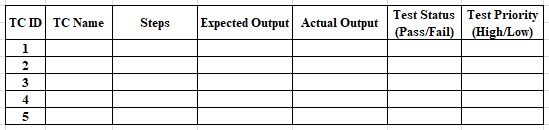
\includegraphics{images/testcases.jpg}
				\caption{Test Cases}
			\end{figure}


%********************************************************************************************
%									Chapter (Outputs/ Results) 
%********************************************************************************************

	\chapter{Outputs/ Results}
	\pagebreak
		DIAGRAMS (n)


%********************************************************************************************
%								Chapter (Conclusion and Future Scope) 
%********************************************************************************************

	\chapter{Conclusion and Future Scope}
	\pagebreak	
		\section{Conclusion}
		\lipsum[4]
		
		\section{Future Scope}
		\begin{itemize}
			\item Point
			\item Point
			\item Point
			\item Point
		\end{itemize}

%********************************************************************************************
%										Chapter (References) 
%********************************************************************************************
	
	\addcontentsline{toc}{chapter}{References}
	\chapter*{References}
	\pagebreak
		References
	\pagebreak
	
%********************************************************************************************
%										Annexure Section
%********************************************************************************************
	
	\renewcommand{\appendixname}{Annexure} %To rename "Appendix" to "Annexure"
	
	\begin{appendices}
		
	\chapter{Laboratory Assignments on Project Analysis of Algorithmic Design.}
	\pagebreak
	\vspace*{0.5cm}
		
	To develop the problem under consideration and justify feasibilty using concepts
	of knowledge canvas and IDEA Matrix.
	\vspace*{0.5cm}
	
		\begin{table}[h]
			\centering
			\renewcommand{\arraystretch}{1.5}
			\begin{tabular}{|c|c|c|c|}
				\hline
				\textbf{I} & \textbf{D} & \textbf{E} & \textbf{A} \\
				\hline
				Increase & Drive & Educate & Accelerate \\
				\hline
				Improve & Deliver & Evaluate & Associate \\
				\hline
				Ignore & Decrease & Eliminate & Avoid \\
				\hline
			\end{tabular}
		\caption{IDEA Matrix}
		\end{table}
		
		\begin{itemize}
			\item \textbf{Feasibility Study :} The main aim of feasibility study is to check is if indexing of keywords are processed properly. The feasibility study activity involves the anal-ysis of the problem and collection of all relevant information relating to the accuracy of authentication in the system. Feasibility study also involves for time complexity of system.
			
			\item \textbf{Options Assessed :} In absence of failure of authentication User cannot proceed data from the System.
			
			\item \textbf{Technical Feasibility :} Technical feasibility assesses whether given system can be developed with the technology that is currently available in the technical marketplace. It finds out technical requirements of the proposed system and matches them against the technical expertise available within the
			organization. The analysts determine whether the in-house technical	capabilities need to be upgrade or new technical resources can be hired to fulfill the technical requirements of the project.
			
			\item \textbf{Economic Feasibility :} Economic analysis is the most frequently used technique for evaluat-ing the effectiveness of a proposed system. More commonly known as Cost / Benefit analysis, the procedure is to determine the benefits and savings that are expected from a proposed system and compare them
			with costs. If benefits outweigh costs, a decision is taken to design and
			implement the system. Otherwise, further justification or alternative in the proposed system will have to be made if it is to have a chance of being approved. This is an outgoing effort that improves in accuracy
			at each phase of the system life cycle.
			
			\item \textbf{Operational Feasibility :} This is mainly related to human organizational aspects. The points to be considered are: This feasibility study is carried out by a small group of people who are familiar with information system technique and are skilled in system analysis and design process.
		\end{itemize}
					
	\chapter{Laboratory Assignments on Project Quality and Reliability Testing of Project Design.}
	\pagebreak
	\vspace*{0.5cm}
		
		\begin{itemize}
			\item Use of divide and conquer strategies to exploit distributed/parallel/concurrent
			processing of the above to identify object, morphisms, overloading in functions
			(if any), and functional relations and any other dependencies (as per requirements).
			It can include Venn diagram, state diagram, function relations,
			i/o relations; use this to derive objects, morphism, overloading
			\item Use of above to draw functional dependency graphs and relevant Software
			modeling methods, techniques including UML diagrams or other necessities
			using appropriate tools.
			\item Testing of project problem statement using generated test data (using mathematical
			models, GUI, Function testing principles, if any) selection and appropriate
			use of testing tools, testing of UML diagram’s reliability. Write also test
			cases [Black box testing] for each identified functions. You can use Mathematica
			or equivalent open source tool for generating test data.
		\end{itemize}
		
		
		\section{Mathematical Equation}
		Equations.
		\section{Sequence Diagram}
		DIAGRAM (1)
		\section{Deployment Diagram}
		DIAGRAM (1)
		
		\chapter{Project Plan.}
		\pagebreak
		\vspace*{0.5cm}
		Project Plan can be created using planner or alike project management tool, we have used Microsoft Excel to create one.
		
		\begin{figure}[h]
			\centering
			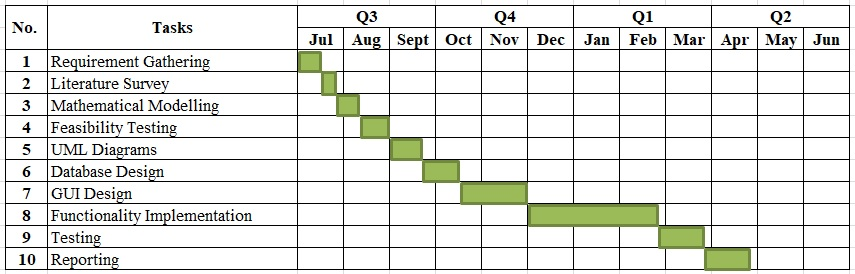
\includegraphics[scale=0.75]{images/project plan.jpg}
			\caption{Project Plan }
		\end{figure}
		
	\chapter{Reviewer's Comments on Submitted Paper.}
	\pagebreak
	\vspace*{0.5cm}
		
		\begin{enumerate}
			\item Paper Title : Your Awesome Project Report Title
			\item Name of the Conference/Journal where paper submitted :
			\item Paper Accepted/Rejected : Accepted.
			\item Review comments by reviewer : -
			\item Corrective actions if any : -
		\end{enumerate}
		
	\chapter{Plagiarism Report.}
	\pagebreak
	\vspace*{0.5cm}
	Plagiarism report as stated by the website https://searchenginereports.net/plagiarism-checker for each module :
		
		\begin{enumerate}
			\item Abstract
			\item Synopsis
			\item Introduction
			\item Problem Definition and Scope
			\item Project Plan
			\item Software Requirement Specification
		\end{enumerate}
		
		\begin{figure}[h]
			\centering
			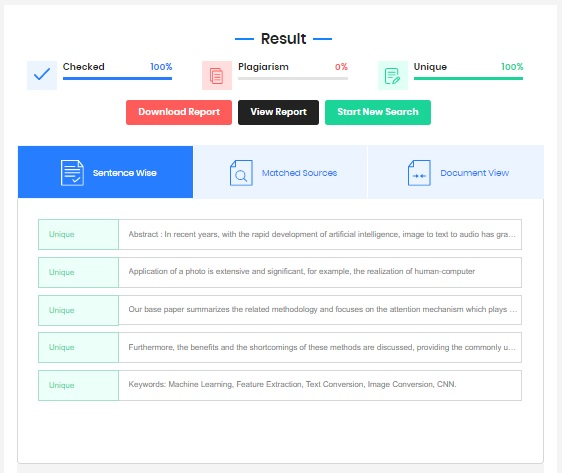
\includegraphics{images/plagiarism report.jpg}
			\caption{Plagiarism Report}
		\end{figure}		
		
		\chapter{TERM-II Project Laboratory Assignments.}
		\pagebreak
		\vspace*{0.5cm}
		\section{Software(s) Installation}
		\textbf{Software  1:}
		\begin{description}
			\item [Step 1 :] 
			\item [Step 2 :] 
			\item [Step 3 :] 
		\end{description}
		\vspace{\baselineskip}
		
		\flushleft
		\textbf{Software  2:}
		\begin{description}
			\item [Step 1 :] 
			\item [Step 2 :] 
			\item [Step 3 :] 
		\end{description}
				
		\section{GUI/Interface}
		GUI is developed using HTML5 and CSS.
		
		\section{Test Cases}
		\begin{figure}[h]
			\centering
			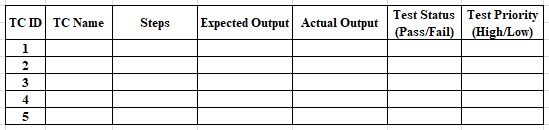
\includegraphics{images/testcases.jpg}
			\caption{Test Cases}
		\end{figure}
		
	\chapter{Information of Project Group Members.}
	\pagebreak
	\vspace*{0.5cm}
	Below are the details of the project group members : \\
	\textbf{Student 1 Details :}
	\vspace{0.5cm}
		
		\centering
		\begin{tabular}{ll}
			\multirow{2}{*}{
\includegraphics[scale=0.05]{images/student1.jpg}} & \textbf{Name :} Student 1 \\
			& \textbf{Address :} Pune, Maharashtra.  \\
			& \textbf{Mobile no. :} +91 9876543210  \\
			& \textbf{E-mail :} student1email@gmail.com  \\
			& \textbf{Birthdate :} 20/10/2000  \\
			& \textbf{Placement Details :} NVIDIA Graphics Pvt. Ltd.  \\
		\end{tabular}
		
		\flushleft
		\textbf{Student 2 Details :}
		\vspace{0.5cm}
		
		\centering
		\begin{tabular}{ll}
			\multirow{2}{*}{
\includegraphics[scale=0.05]{images/student2.jpg}} & \textbf{Name :} Student 2 \\
			& \textbf{Address :} Pune, Maharashtra.  \\
			& \textbf{Mobile no. :} +91 9876543210  \\
			& \textbf{E-mail :} student1email@gmail.com  \\
			& \textbf{Birthdate :} 20/10/2000  \\
			& \textbf{Placement Details :} NVIDIA Graphics Pvt. Ltd.  \\
		\end{tabular}
		
		\flushleft
		\textbf{Student 3 Details :}
		\vspace{0.5cm}
		
		\centering
		\begin{tabular}{ll}
			\multirow{2}{*}{
\includegraphics[scale=0.05]{images/student3.jpg}} & \textbf{Name :} Student 3 \\
			& \textbf{Address :} Pune, Maharashtra.  \\
			& \textbf{Mobile no. :} +91 9876543210  \\
			& \textbf{E-mail :} student1email@gmail.com  \\
			& \textbf{Birthdate :} 20/10/2000  \\
			& \textbf{Placement Details :} NVIDIA Graphics Pvt. Ltd.  \\
		\end{tabular}
		
		\flushleft
		\textbf{Student 4 Details :}
		\vspace{0.5cm}
		
		\centering
		\begin{tabular}{ll}
			\multirow{2}{*}{
\includegraphics[scale=0.05]{images/student4.jpg}} & \textbf{Name :} Student 4 \\
			& \textbf{Address :} Pune, Maharashtra.  \\
			& \textbf{Mobile no. :} +91 9876543210  \\
			& \textbf{E-mail :} student1email@gmail.com  \\
			& \textbf{Birthdate :} 20/10/2000  \\
			& \textbf{Placement Details :} NVIDIA Graphics Pvt. Ltd.  \\
		\end{tabular}
		
	\end{appendices}
		
\end{document}	

%********************************************************************************************
%								End of Report
%********************************************************************************************
